\documentclass[12pt]{article}
\usepackage[utf8]{inputenc}
\usepackage[spanish]{babel}
\usepackage{graphicx}
\usepackage{float}
\title{Práctica 2\\Programación Evolutiva}
\author{Grupo 01\\Rafael Fernández López\\Ángel Valero Picazo}
\date{}

\pdfinfo
{
  /Title       (PRACTICA2-PE)
  /Author      (RAFAEL FERNANDEZ LOPEZ, ANGEL VALERO PICAZO)
}

\begin{document}

\maketitle
\newpage
\newpage
\tableofcontents
\newpage

\section{Introducción}

	En esta memoria se van a estudiar los diferentes métodos de selección, cruce y mutación para poder
    evaluar cuáles se comportan mejor y cuáles son menos precisos a la hora de tratar el problema del
    viajante implementado en esta práctica.

\section{Métodos propios}

	En este apartado se explican los dos métodos propios implementados en la práctica.

\subsection{Cruce propio}

	Este cruce se basa en el algoritmo de ciclos. En el vector se fijan pares cada dos posiciones,
    esos pares fijados se trataran de forma semejante al algoritmo de ciclos, copiando del padre dos
    a dos cada dos posiciones, quedando dos ciudades libres por cada dos ocupadas. Después, se rellenan
    estas posiciones vacías utilizando el algoritmo por orden en la madre.

    De esta manera, no existen repeticiones, y podemos decir que de alguna manera se mantiene un buen resultado, dado que no hay
    demasiada permutación de las ciudades en los hijos, y aún así, se introduce diversidad suficiente
    para innovar y crear nuevos individuos que tengan una muy buena aptitud.

\subsection{Mutación propio}

    Siguiendo la mentalidad de nuestro cruce propio, hemos escrito un tipo de mutación propia que lo
    que hace es intercambiar ciudades de dos en dos y dos a dos.

    Al igual que anteriormente, tenemos un buen compromiso entre innovación y conservación de buenos
    individuos.
    
\section{Estudio de selección por Torneo}

    En este apartado se va a estudiar la selección por torneo, para ello hemos tomado por defecto los
    valores que se exponen en la tabla que se presenta a continuación.

%tabla
\begin{table}[H]
\begin{center}
\begin{tabular}{|cc|} \hline
Tamaño de la Población   & 100  \\  
Número Máximo de Generaciones  &  300 \\
Probabilidad de Cruce & 0.5 \\
Probabilidad de Mutación & 0.15 \\
Porcentaje de Elitismo & 0.02 \\ \hline
\end{tabular}
\end{center}
\end{table}

Estudio de la selección por torneo probando los diferentes métodos de cruce y mutación.

%tabla
\begin{table}[H]
\begin{center}
\begin{tabular}{|ccccc|} \hline
	   & Inserción & Intercambio & Inversión & Propio \\  \hline
PMX 	   &  7657 & 10591 & 8098 & 7581 \\ 
OX 	   & 7418 & 9807 & 7955 & 6142  \\ 
Variante OX & 7269 & 10380 & 7816 & 7573 \\
Ciclos 	   & 7759 & 10330 & 7459 & 8953 \\
ERX 	   & 6649 & 9937 & 6430 & 5550 \\
Ordinal    & 8199 & 9409 & 8057 & 9415 \\
Propio     & 7671 & 10245 & 8906 & 10441 \\  \hline
\end{tabular}
\end{center}
\end{table}

	Se observa referente a los cruces que los que mejores resultados se dan con ERX seguido por OX y su variante OX. En cambio los peores resultados se obtienen con el método de cruce propio.

	Referente a las mutaciones se puede ver como inversión y la mutación propia obtienen generalmente buenos resultados, en contra la que peor se comporta es la de intercambio.

\begin{figure}[H]
\centering
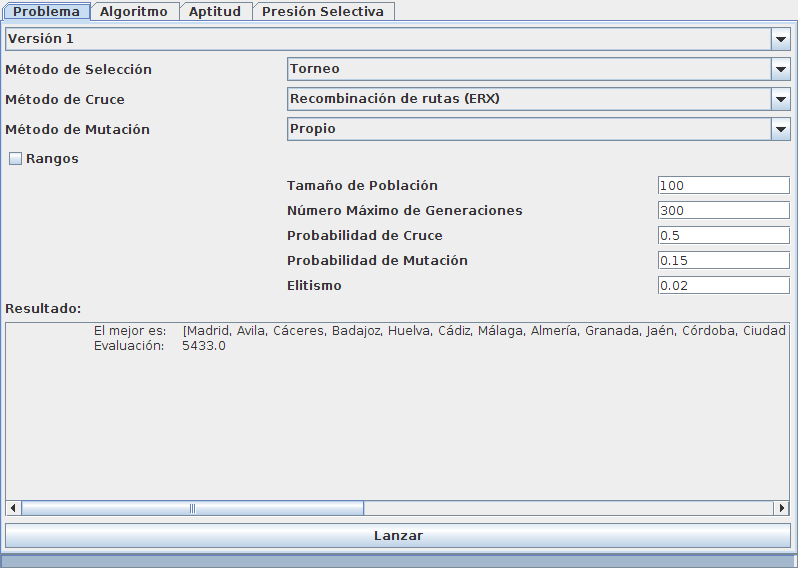
\includegraphics[scale=0.4]{graficas/fig1}
\caption{Captura mejor resultado.}
\end{figure}

\begin{figure}[H]
\centering
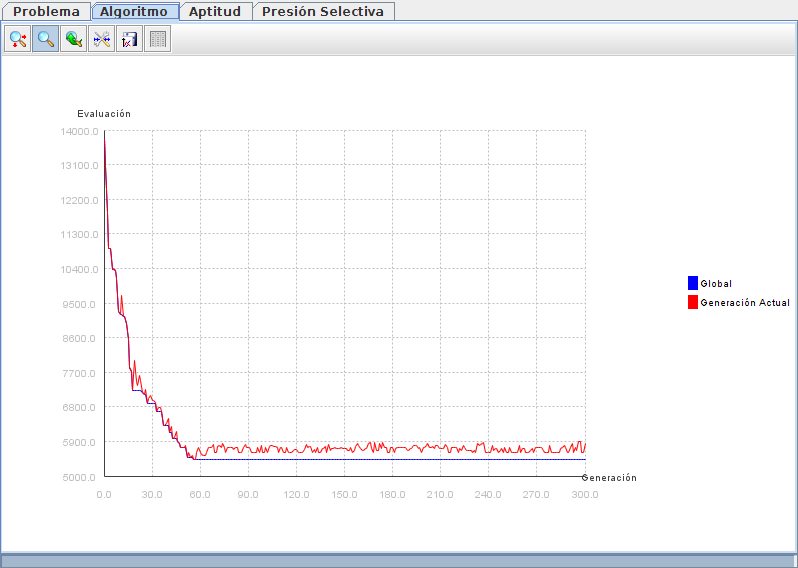
\includegraphics[scale=0.4]{graficas/fig1graf}
\caption{Evaluación}
\end{figure} 

\section{Estudio de selección por Ranking}

A continuación se va a estudiar la selección por ranking, para ello hemos tomado por defecto los valores que anteriormente se han mencionado.	

%tabla
\begin{table}[H]
\begin{center}
\begin{tabular}{|ccccc|} \hline
	   & Inserción & Intercambio & Inversión & Propio \\  \hline
PMX 	   &  8541 & 10231 & 9192 & 7619 \\ 
OX 	   & 9262 & 9988 & 8629 & 8089  \\ 
Variante OX & 8834 & 10332 & 9537 & 7410 \\
Ciclos 	   & 8530 & 10370 & 8208 & 9327 \\
ERX 	   & 8653 & 10470 & 8050 & 7777 \\
Ordinal    & 8990 & 10280 & 9287 & 8536 \\
Propio     & 8763 & 9763 & 8803 & 9936 \\  \hline
\end{tabular}
\end{center}
\end{table}

	Se puede ver que los mejores cruces utilizados el método de selección de ranking siguen siendo ERX,
    OX y su variante, pero ahora destaca el PMX.

	En las mutaciones se repite los resultados anteriores siendo la mejor la propia pero ahora se
    igualan la de inserción e inversión. Como antes la peor sigue siendo la de intercambio.

\begin{figure}[H]
\centering
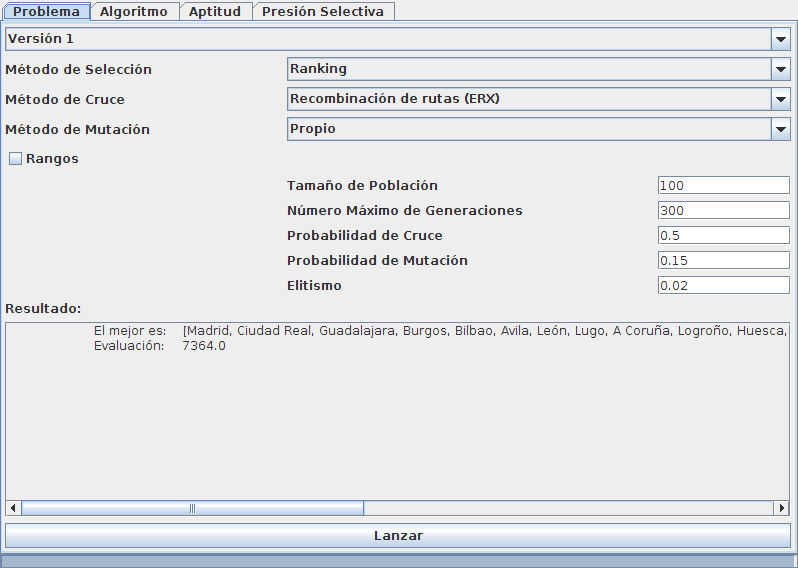
\includegraphics[scale=0.4]{graficas/fig2}
\caption{Captura mejor resultado.}
\end{figure}

\begin{figure}[H]
\centering
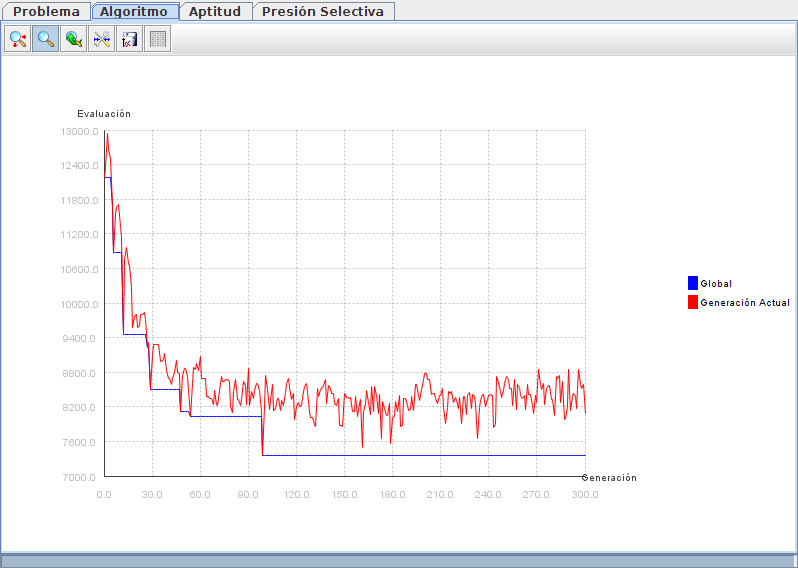
\includegraphics[scale=0.4]{graficas/fig2graf}
\caption{Evaluación}
\end{figure}   

\section{Estudio de selección por Ruleta}	

	 Por último se estudia el método de selección por ruleta, en este caso sólo se ha estudiado con el método de cruce ERX y con sus cuatro correspondientes métodos de mutación.

%tabla
\begin{table}[H]
\begin{center}
\begin{tabular}{|ccccc|} \hline
	   & Inserción & Intercambio & Inversión & Propio \\  \hline
ERX    & 11769 & 11369 & 11807 & 11382 \\  \hline
\end{tabular}
\end{center}
\end{table}

	Como se esperaba por el estudio teórico de dicha selección los valores resultantes no son nada buenos debido probablemente a una convergencia prematura.

	En esta selección no existen diferencias notables entre los diferentes métodos de mutación.

\begin{figure}[H]
\centering
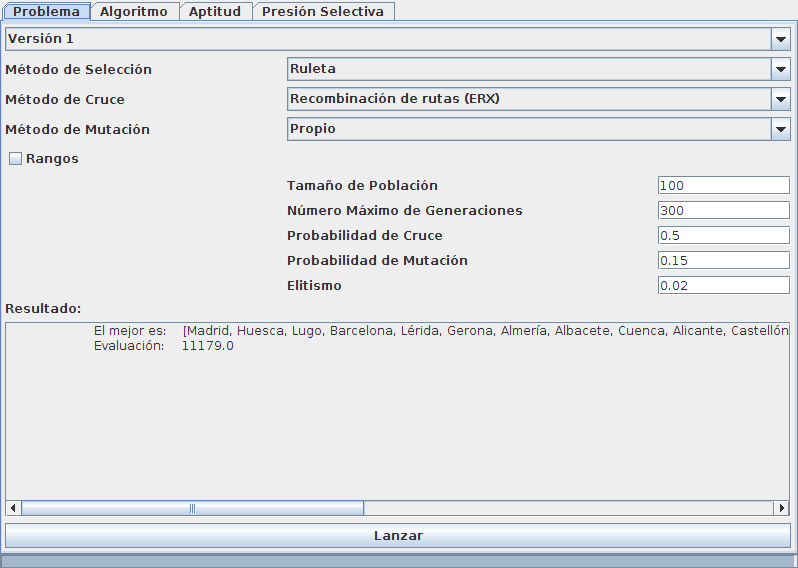
\includegraphics[scale=0.4]{graficas/fig3}
\caption{Captura mejor resultado.}
\end{figure}

\begin{figure}[H]
\centering
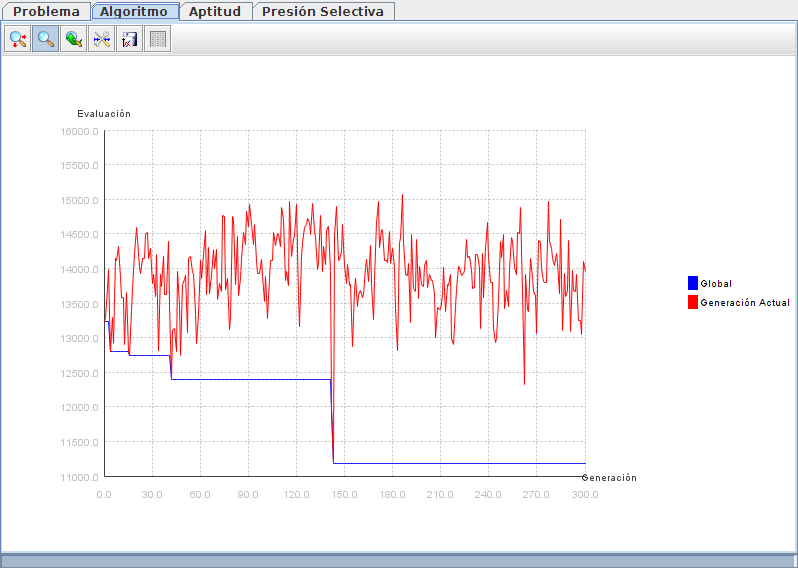
\includegraphics[scale=0.4]{graficas/fig3graf}
\caption{Evaluación}
\end{figure} 

\section{Estudio de los diferentes parámetros del Algoritmo Genético}

	Estudio realizado con selección de torneo, cruce ERX y mutación propia. Se han ido variando los diferentes parámetros, por defecto hemos tomados los siguientes valores:

%tabla
\begin{table}[H]
\begin{center}
\begin{tabular}{|cc|} \hline
Tamaño de la Población   & 100  \\  
Número Máximo de Generaciones  &  300 \\
Probabilidad de Cruce & 0.5 \\
Probabilidad de Mutación & 0.15 \\
Porcentaje de Elitismo & 0.02 \\ \hline
\end{tabular}
\end{center}
\end{table}


\subsection{Tamaño de la Población}

%tabla
\begin{table}[H]
\begin{center}
\begin{tabular}{|ccccc|} \hline
Tamaño	   & 50 & 100 & 150 & 200 \\  \hline
Resultado  &  6415 & 5503 & 5644 & 5498 \\ \hline
\end{tabular}
\end{center}
\end{table}

	Se puede observar como el valor óptimo esta en torno a 100 individuos en el tamaño de población. 

\subsection{Número Máximo de Generaciones}
%tabla
\begin{table}[H]
\begin{center}
\begin{tabular}{|ccccc|} \hline
Num Generaciones  & 100 & 200 & 300 & 400 \\  \hline
Resultado  &  5771 & 5419 & 5419 & 5733 \\ \hline
\end{tabular}
\end{center}
\end{table}	

	En este caso el número máximo de generaciones está en torno al intervalo 200-300 el valor óptimo.

\subsection{Probabilidad de Cruce}
%tabla
\begin{table}[H]
\begin{center}
\begin{tabular}{|ccccc|} \hline
Probabilidad   & 0.2 & 0.4 & 0.5 & 0.7 \\  \hline
Resultado  &  6198 & 5668 & 5611 & 5480 \\ \hline
\end{tabular}
\end{center}
\end{table}

	La probabilidad de cruce adecuada para este problema converge entre 0.5 y 0.7.

\subsection{Probabilidad de Mutación}
%tabla
\begin{table}[H]
\begin{center}
\begin{tabular}{|ccccc|} \hline
Probabilidad   & 0.05 & 0.1 & 0.15 & 0.2 \\  \hline
Resultado  &  5713 & 5668 & 5514 & 5703 \\ \hline
\end{tabular}
\end{center}
\end{table}

	La mejor probabilidad de mutación se sitúa alrededor de 0.15.

\subsection{Porcentaje de Elitismo}
%tabla
\begin{table}[H]
\begin{center}
\begin{tabular}{|ccccc|} \hline
Porcentaje   & 0.0 & 0.02 & 0.1 & 0.3 \\  \hline
Resultado  &  6795 & 5368 & 5514 & 5946 \\ \hline
\end{tabular}
\end{center}
\end{table}

	Se observa como al eliminar el elitismo poniéndolo a 0, el resultado empeora notablemente, el mejor porcentaje de elitismo se encuentra en torno a 0.02.


\section{Conclusiones}

Primero se van a exponer las conclusiones relacionadas con los diferentes métodos de selección.

La selección por ruleta permite a los mejores individuos ser elegidos con una mayor probabilidad, pero también permite a los peores individuos ser elegidos, lo cual ayuda a mantener la diversidad de la población.
Un problema que hemos observado con los diferentes estudios realizados es que dicha selección hace perder diversidad y puede conducir a una convergencia prematura ya que la mayor parte de los individuos seleccionados serán una copia de los pocos predominantes.

En la selección por ranking los individuos se ordenan según su puntuación y luego son asignados con una segunda medida de puntuación, inversamente proporcional a su posición en el ranking. Los individuos son seleccionados proporcionalmente a esta probabilidad. Este método cómo se observa en los estudios realizados disminuye el riesgo de convergencia prematura que se produce cuando se utiliza selección de ruleta. Comentar que de los tres métodos implementados para la selección es el mas eficiente en cuanto a tiempo.

Por ultimo la selección por torneo se efectúa mediante una comparación entre un pequeño subconjunto de individuos elegidos al azar desde la población.
Los beneficios de este tipo de selección son la velocidad de aplicación ya que no es necesario evaluar ni comparar la totalidad de la población y la capacidad de prevenir la convergencia prematura. La principal desventaja es la necesidad de establecer el parámetro correspondiente al tamaño del subconjunto , en nuestro caso son 3 individuos y da buenos resultados.

Sobre las mejoras introducidas en la práctica hay que destacar el elitismo, método que copia los mejores individuos a la
próxima generación. El elitismo puede aumentar rápidamente hacia buenos individuos, ya que evita perder la mejor solución encontrada. Sin embargo,
es posible que este método haga converger rápidamente a un óptimo local.

También, para guiar correctamente al algoritmo, ha sido necesario escalar y adaptar la aptitud. De esta forma,
al principio del algoritmo, tenemos una visión muy global de todos los individuos de las generaciones. Según
avanza el algoritmo, esta aptitud es adaptada y escalada de tal manera que haya menos espacio entre los individuos,
haciendo `zoom' en los resultantes, de manera que nos `centramos' en una determinada zona al final del algoritmo.

Gracias a esto, conservamos una buena diversidad al principio (siempre y cuando no hablemos del método de selección de la Ruleta), y nos vamos centrando más al final del algoritmo.

\end{document}
